\documentclass[11pt,a4paper]{article}

\usepackage[utf8]{inputenc}
\usepackage[T1]{fontenc}
\usepackage{amsmath, amssymb}
\usepackage{geometry}
\usepackage{booktabs}
\usepackage{array}
\usepackage{enumitem}
\usepackage{hyperref}
\usepackage{algorithm}
\usepackage{algpseudocode}
\usepackage{xcolor}
\usepackage{fancyhdr}
\usepackage{listings}
\usepackage{tikz}
\usetikzlibrary{positioning}

% Nota: el paquete babel con el idioma espanol no esta disponible en este
% entorno de compilacion (falta texlive-lang-spanish). Se traducen a mano
% las pocas cadenas automaticas que usa el documento (p. ej. "Resumen").
% Si se compila en Overleaf o con una instalacion completa de TeX Live,
% se puede agregar \usepackage[spanish]{babel} sin que cambie el resultado.
\renewcommand{\abstractname}{Resumen}

\geometry{margin=2.5cm}
\hypersetup{colorlinks=true, linkcolor=blue, urlcolor=blue, citecolor=blue}

\pagestyle{fancy}
\fancyhf{}
\lhead{Algoritmos Avanzados -- Avance 2}
\rhead{Grupo 1 -- Cobertura de Vértices}
\cfoot{\thepage}

\lstset{
	basicstyle=\ttfamily\small,
	breaklines=true,
	frame=single,
	columns=fullflexible,
	backgroundcolor=\color{gray!8}
}

\title{
	\vspace{-1.5cm}
	\textbf{Diseño Algorítmico y Plan de Validación} \\
	\large Cobertura de Vértices para la ubicación de sistemas de detección de intrusos
}
\author{
	Grupo 1 \\
	\small Universidad Nacional de San Antonio Abad del Cusco \\
	\small Escuela Profesional de Ingeniería Informática y de Sistemas \\
	\small Asignatura: Algoritmos Avanzados \\
	\small Docente: Héctor Eduardo Ugarte Rojas
}
\date{Semestre académico 2026-2 \\ Avance 2: Diseño algorítmico y plan de validación}

\begin{document}
\maketitle
\thispagestyle{fancy}

\begin{abstract}
\noindent
Se presenta el diseño preliminar del sistema: módulos, estructuras de datos, flujo de
información, formato de archivos, pseudocódigo y análisis de complejidad de los algoritmos
implementados. Se resuelve paso a paso una instancia pequeña usando el sistema real (no solo
a mano), se describe el plan de pruebas (básicas, límite y adversarias) ya implementado, el
criterio de verificación de salidas, las herramientas candidatas evaluadas con sus criterios
de selección, y las métricas previstas para la comparación experimental. Todo el código
referido en este documento corresponde al repositorio Git del proyecto y es ejecutable.
\end{abstract}

% ======================================================
\section{Arquitectura y módulos del sistema}

El sistema se organiza en módulos con responsabilidades separadas, siguiendo el principio de
que la lógica algorítmica no debe depender de cómo se presenta o se invoca:

\begin{center}
\begin{tabular}{p{2.6cm}p{3.6cm}p{7.5cm}}
	\toprule
	\textbf{Módulo} & \textbf{Archivo} & \textbf{Responsabilidad} \\
	\midrule
	Grafo & \texttt{src/graph.py} & Estructura de datos, carga/guardado de instancias, generadores sintéticos \\
	Solver & \texttt{src/solver.py} & Los tres algoritmos (greedy, matching, exacto) \\
	Verificación & \texttt{src/verify.py} & Validación de coberturas y cálculo de métricas \\
	Pruebas & \texttt{tests/} & Casos básicos, límite y adversarios (pytest) \\
	Experimentos & \texttt{experiments/\allowbreak compare.py} & Comparación empírica y exportación a CSV \\
	Prototipo/demo & \texttt{demo.py} & Interfaz de línea de comandos para la demostración \\
	\bottomrule
\end{tabular}
\end{center}

\subsection{Flujo de información}

\begin{center}
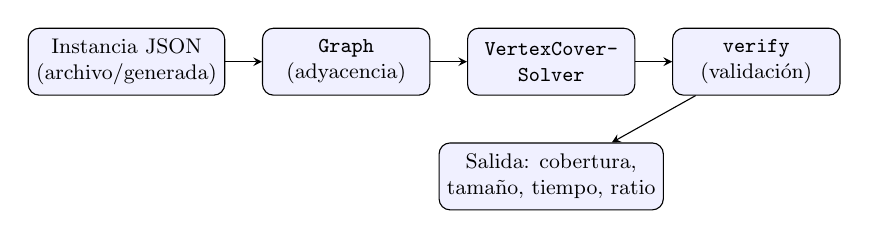
\begin{tikzpicture}[
	scale=0.85, transform shape,
	node distance=0.55cm and 0.55cm,
	box/.style={draw, rounded corners, align=center, minimum width=2.5cm, minimum height=1cm, fill=blue!6, font=\small},
	>=stealth
]
	\node[box] (file) {Instancia JSON\\(archivo/generada)};
	\node[box, right=of file] (graph) {\texttt{\small Graph}\\(adyacencia)};
	\node[box, right=of graph] (solver) {\texttt{\small VertexCover-}\\\texttt{\small Solver}};
	\node[box, right=of solver] (verify) {\texttt{\small verify}\\(validación)};
	\node[box, below=0.7cm of solver] (out) {Salida: cobertura,\\tamaño, tiempo, ratio};

	\draw[->] (file) -- (graph);
	\draw[->] (graph) -- (solver);
	\draw[->] (solver) -- (verify);
	\draw[->] (verify) -- (out);
\end{tikzpicture}
\end{center}

\subsection{Estructura de datos elegida}

Se usa una \textbf{lista de adyacencia} (\texttt{dict[vértice, set[vértice]]}) en lugar de una
matriz de adyacencia. Justificación:
\begin{itemize}
	\item Las redes reales son dispersas ($|E| \ll |V|^2$), por lo que una matriz desperdiciaría
	memoria: $O(V^2)$ vs. $O(V+E)$ de la lista de adyacencia.
	\item Obtener el grado de un vértice es $O(1)$ (tamaño del conjunto de vecinos), operación
	central en el algoritmo greedy.
	\item Insertar/eliminar una arista es $O(1)$ amortizado gracias al uso de \texttt{set}.
\end{itemize}

\subsection{Formato de archivo de instancia}

Las instancias se guardan en JSON, elegido por ser legible por humanos, nativo en Python y
fácil de versionar en Git (diffs claros por línea):

\begin{lstlisting}
{
  "name": "example_small",
  "description": "...",
  "vertices": ["A", "B", "C", "D", "E", "F"],
  "edges": [["A","B"], ["A","C"], ["A","D"], ["B","C"], ["D","E"], ["E","F"]]
}
\end{lstlisting}

% ======================================================
\section{Pseudocódigo y análisis de complejidad}

\subsection{Greedy por grado}
\begin{algorithm}[H]
\caption{\texttt{greedy\_degree\_vertex\_cover}}
\begin{algorithmic}[1]
\State $E' \gets E$ \Comment{aristas pendientes}
\State $C \gets \emptyset$
\While{$E' \neq \emptyset$}
	\State calcular $\deg_{E'}(v)$ para cada $v$ incidente en $E'$
	\State $v^{*} \gets \arg\max_v \deg_{E'}(v)$
	\State $C \gets C \cup \{v^{*}\}$
	\State $E' \gets E' \setminus \{(u,w) \in E' : u = v^{*} \lor w = v^{*}\}$
\EndWhile
\State \Return $C$
\end{algorithmic}
\end{algorithm}

\textbf{Complejidad:} en la implementación actual (\texttt{src/solver.py}), cada iteración
recorre las aristas restantes para recalcular grados: $O(E)$ por iteración, hasta $O(V)$
iteraciones en el peor caso $\Rightarrow O(V \cdot E)$. Puede optimizarse a
$O((V+E)\log V)$ manteniendo una cola de prioridad con grados actualizados perezosamente;
queda identificado como mejora para la Entrega 2.

\textbf{Garantía de aproximación:} ninguna cota fija demostrable en el peor caso general
(existen instancias donde el greedy se aleja más del óptimo que el matching maximal);
en la práctica, sobre las instancias probadas, el ratio empírico se mantuvo entre 1.0x y
1.2x (ver Sección~\ref{sec:resultados}).

\subsection{Matching maximal (2-aproximación)}
\begin{algorithm}[H]
\caption{\texttt{maximal\_matching\_vertex\_cover}}
\begin{algorithmic}[1]
\State $E' \gets E$
\State $C \gets \emptyset$
\While{$E' \neq \emptyset$}
	\State tomar $(u,v) \in E'$ \Comment{orden canónico, ver Nota de reproducibilidad}
	\State $C \gets C \cup \{u, v\}$
	\State $E' \gets E' \setminus \{(a,b) \in E' : a \in \{u,v\} \lor b \in \{u,v\}\}$
\EndWhile
\State \Return $C$
\end{algorithmic}
\end{algorithm}

\textbf{Complejidad:} $O(V+E)$: cada arista se visita y se elimina a lo sumo una vez del
conjunto de pendientes.

\textbf{Garantía de aproximación (demostración breve):} las aristas elegidas $(u_1,v_1),
(u_2,v_2), \dots$ no comparten extremos (forman un \emph{matching}), porque cada elección
elimina todas las aristas incidentes a los vértices recién agregados. Por lo tanto, toda
cobertura válida —incluida la óptima— debe contener al menos un extremo de cada una de esas
aristas (ya que son disjuntas, ningún vértice puede "cubrir" dos de ellas a la vez). Si el
matching tiene $k$ aristas, entonces $|C^{*}| \geq k$. El algoritmo agrega $2k$ vértices, por
lo tanto $|C_{\text{match}}| = 2k \leq 2 \cdot |C^{*}|$.

\subsection{Exacto (fuerza bruta de referencia)}
\begin{algorithm}[H]
\caption{\texttt{exact\_vertex\_cover\_bruteforce}}
\begin{algorithmic}[1]
\For{$k = 1$ \textbf{hasta} $|V|$}
	\For{cada subconjunto $S \subseteq V$ con $|S| = k$}
		\If{$S$ cubre todas las aristas de $E$}
			\State \Return $S$
		\EndIf
	\EndFor
\EndFor
\end{algorithmic}
\end{algorithm}

\textbf{Complejidad:} $O\left(\binom{V}{k^{*}} \cdot E\right)$ en el peor caso, acotado
superiormente por $O(2^{V} \cdot E)$. Por esta razón \texttt{exact\_vertex\_cover\_bruteforce}
rechaza instancias de más de 20 vértices (parámetro configurable) y lanza
\texttt{ValueError} en vez de ejecutarse indefinidamente. Los datos de la
Sección~\ref{sec:resultados} confirman el crecimiento exponencial esperado.

\textbf{Nota de reproducibilidad.} Durante la implementación se detectó que iterar
directamente sobre un \texttt{set()} de aristas en Python produce un orden distinto en cada
ejecución del proceso (por la aleatorización del hash de los \textit{strings},
\texttt{PYTHONHASHSEED}), lo que rompía la reproducibilidad exigida por el proyecto: dos
corridas de un mismo algoritmo sobre la misma instancia podían devolver coberturas válidas
pero de tamaño distinto. Se corrigió introduciendo \texttt{VertexCoverSolver.\_sorted\_edges()},
que fija un orden canónico y determinístico para los desempates del greedy y la elección
"arbitraria" del matching. Ver el commit \texttt{fix: hacer deterministas greedy y matching
maximal} en el historial del repositorio.

% ======================================================
\section{Instancia resuelta paso a paso con el sistema real}

Se ejecuta \texttt{demo.py} sobre la instancia \texttt{data/instances/example\_small.json}
(la misma mini-red de 6 routers del Avance 1):

\begin{lstlisting}[language=bash]
$ python demo.py --instance data/instances/example_small.json --algorithm all
\end{lstlisting}

\textbf{Salida real del sistema:}
\begin{lstlisting}
Cargado: instancia 'data/instances/example_small.json'
  |V| = 6   |E| = 6

[Greedy por grado]
  Cobertura: ['A', 'B', 'E']
  Tamano: 3
  Valida: SI
  Tiempo: 0.034 ms

[Matching maximal (2-aprox)]
  Cobertura: ['A', 'B', 'D', 'E']
  Tamano: 4
  Valida: SI
  Tiempo: 0.018 ms

[Exacto (fuerza bruta)]
  Cobertura: ['A', 'B', 'E']
  Tamano: 3
  Valida: SI
  Tiempo: 0.031 ms

Ratios de aproximacion frente al optimo:
  Greedy por grado: 1.000x
  Matching maximal (2-aprox): 1.333x
\end{lstlisting}

El resultado coincide exactamente con la traza manual del Avance 1 (greedy = $\{A,B,E\}$,
tamaño 3; matching = $\{A,B,D,E\}$, tamaño 4), lo que valida que la implementación respeta
el pseudocódigo acordado.

% ======================================================
\section{Plan de pruebas}

El plan de pruebas ya está implementado en \texttt{tests/} (27 casos, \texttt{pytest}) y se
organiza en las tres categorías pedidas:

\begin{center}
\small
\begin{tabular}{p{2.1cm}p{9.3cm}p{2.8cm}}
	\toprule
	\textbf{Categoría} & \textbf{Casos} & \textbf{Archivo} \\
	\midrule
	Básicos    & Construcción del grafo; instancia del Avance 1 (resultado exacto esperado);
	             triángulo $K_3$ (óptimo conocido = 2). & \texttt{test\_graph.py},
	             \texttt{TestCasos\-Basicos} \\[2pt]
	Límite     & Grafo sin aristas; una sola arista (evidencia directa de la cota 2x);
	             vértices aislados; grafo completo $K_4$ (óptimo $=n-1$); componentes
	             desconectadas; fuerza bruta rechazando instancias $>20$ vértices. &
	             \texttt{TestCasos\-Limite} \\[2pt]
	Adversarios & Grafo estrella (greedy óptimo, matching subóptimo pero válido);
	             verificación parametrizada en 10 grafos aleatorios de que el matching
	             maximal nunca supera $2\times$ el óptimo; verificación de que ninguna
	             arista queda sin cubrir. & \texttt{TestCasos\-Adversarios} \\
	\bottomrule
\end{tabular}
\end{center}
\normalsize

\subsection{Criterio de verificación de salidas}
Ninguna prueba confía únicamente en el \emph{tamaño} de la cobertura devuelta. Toda salida
se valida con \texttt{is\_vertex\_cover(graph, cover)} (\texttt{src/verify.py}), que
recorre todas las aristas del grafo y confirma que cada una tenga al menos un extremo en la
cobertura. Esto es intencional: un algoritmo con un error de implementación podría devolver
un conjunto del tamaño "esperado" sin que efectivamente cubra el grafo, y una prueba que
solo comparara tamaños no lo detectaría.

\begin{lstlisting}[language=bash]
$ pytest tests/ -v
...
======================== 27 passed in 0.04s =========================
\end{lstlisting}

% ======================================================
\section{Herramientas candidatas y criterios de selección}

\begin{center}
\begin{tabular}{p{2.9cm}p{4.8cm}p{6.5cm}}
	\toprule
	\textbf{Necesidad} & \textbf{Candidatas} & \textbf{Criterio de selección} \\
	\midrule
	Pruebas unitarias &
		\texttt{pytest} vs. \texttt{unittest} (estándar) &
		\texttt{pytest} elegido: sintaxis de \texttt{assert} plano (más legible), soporte
		nativo de parametrización (\texttt{@pytest.mark.parametrize}, usado en las pruebas
		adversarias), amplia adopción y documentación. \\
	Manejo y visualización de grafos &
		\texttt{NetworkX} vs. implementación propia pura &
		Implementación propia elegida para el núcleo (control total sobre la complejidad,
		requisito pedagógico del curso); \texttt{NetworkX} queda como candidata para
		visualización y para contrastar resultados en la Entrega 2. \\
	Solver exacto escalable &
		\texttt{PuLP} vs. \texttt{OR-Tools} &
		\texttt{PuLP} preferido para la siguiente etapa: instala el solver CBC junto con el
		paquete (sin dependencias del sistema), API declarativa simple para la formulación
		ILP estándar de Vertex Cover, documentación suficiente para una formulación de este
		tamaño. \texttt{OR-Tools} se descarta por ahora por una curva de aprendizaje mayor
		para el beneficio adicional que aporta en instancias de este tamaño. \\
	Datos y gráficos &
		\texttt{pandas} + \texttt{matplotlib} &
		Estándar de facto, documentación extensa, suficiente para el volumen de datos de
		este proyecto (decenas a cientos de filas). \\
	\bottomrule
\end{tabular}
\end{center}

Criterios generales aplicados a todas las decisiones: (1) facilidad de instalación sin
dependencias del sistema operativo, (2) calidad y vigencia de la documentación oficial,
(3) curva de aprendizaje razonable para el tiempo disponible, (4) adopción/soporte de la
comunidad, (5) que no añada complejidad innecesaria al núcleo algorítmico (ver "Prioridad
del proyecto", instrucción adicional 5 de la guía).

% ======================================================
\section{Métricas previstas para la comparación}

\begin{itemize}
	\item \textbf{Ratio de aproximación empírico}: $|C_{\text{algoritmo}}| / |C^{*}|$,
	calculado por \texttt{verify.approximation\_ratio}. Es la métrica central: mide qué tan
	lejos queda cada algoritmo del óptimo en la práctica, más allá de su cota teórica.
	\item \textbf{Tiempo de ejecución} (ms), medido con \texttt{time.perf\_counter()} tanto en
	\texttt{demo.py} como en \texttt{experiments/compare.py}.
	\item \textbf{Escalabilidad}: tiempo y ratio en función de $|V|$, para caracterizar cómo
	degrada cada algoritmo al crecer la instancia (ver resultados preliminares abajo).
	\item (Entrega 2) \textbf{Uso de memoria}, pendiente de instrumentar.
\end{itemize}

% ======================================================
\section{Resultados experimentales preliminares}
\label{sec:resultados}

Primera corrida de \texttt{experiments/compare.py}: grafos aleatorios $G(n, 0.3)$,
$n \in \{6,8,10,12,14,16,18\}$, semilla fija por tamaño (reproducible).

\begin{center}
\begin{tabular}{rrrrrr}
	\toprule
	$n$ & $|E|$ & óptimo & greedy (ratio) & matching (ratio) & $t_{\text{exacto}}$ (ms) \\
	\midrule
	6  & 3  & 2  & 2 (1.00x)  & 4 (2.00x)  & 0.02 \\
	8  & 10 & 4  & 4 (1.00x)  & 6 (1.50x)  & 0.06 \\
	10 & 13 & 5  & 6 (1.20x)  & 10 (2.00x) & 0.31 \\
	12 & 19 & 5  & 5 (1.00x)  & 10 (2.00x) & 0.97 \\
	14 & 35 & 9  & 9 (1.00x)  & 12 (1.33x) & 9.08 \\
	16 & 33 & 9  & 9 (1.00x)  & 14 (1.56x) & 29.61 \\
	18 & 52 & 12 & 12 (1.00x) & 16 (1.33x) & 173.90 \\
	\bottomrule
\end{tabular}
\end{center}

\textbf{Observaciones preliminares:}
\begin{itemize}
	\item El tiempo del algoritmo exacto crece de forma visiblemente exponencial incluso en
	este rango pequeño (factor $\approx 6\times$ entre $n{=}16$ y $n{=}18$), confirmando la
	cota $O(2^V \cdot E)$ y justificando la necesidad de una alternativa ILP para la Entrega 2.
	\item El greedy iguala al óptimo en 6 de las 7 instancias; solo se desvía (ratio 1.2x) en
	$n{=}10$.
	\item El matching maximal se mantiene siempre dentro de su cota teórica (máximo observado:
	2.0x, exactamente el límite superior), pero nunca superó al greedy en estas instancias.
	\item Estos resultados son preliminares (densidad fija $p=0.3$, un solo tipo de grafo
	aleatorio); la Entrega 2 ampliará el experimento a distintas densidades y a la topología
	tipo backbone (Barabási-Albert) ya disponible en \texttt{data/instances/network\_backbone\_18.json}.
\end{itemize}

% ======================================================
\section{Conclusiones del avance}

El diseño del sistema está implementado y verificado: estructura de grafo eficiente para
redes dispersas, los tres algoritmos acordados funcionando y validados contra la traza
manual del Avance 1, un plan de pruebas de 27 casos que cubre los escenarios básicos, límite
y adversarios exigidos, y un primer experimento reproducible que ya deja ver el
comportamiento esperado de cada algoritmo. El hallazgo del bug de no-determinismo (y su
corrección) se documenta como evidencia concreta de aprendizaje autónomo y pensamiento
crítico durante el desarrollo. Queda pendiente para la Entrega 2: incorporar el solver ILP
como referencia escalable, ampliar la metodología experimental a más densidades y topologías,
y optimizar la complejidad del greedy con una cola de prioridad.

\end{document}
